\chapter{Evaluation}\label{chap:evaluation}
FlyTrap imposes an overhead to vanilla MQTT brokers. It is vital to ensure that added layer of security does not severely impact operation of the broker, as MQTT is a time-sensitive protocol, requiring frequent and rapid responses. In this chapter, I will design experiments to measure latency caused by FlyTrap, operation cost on public blockchain and reflect back to requirements (\& user stories) to ensure that FlyTrap fulfills all of the specified needs. In the end, I will reflect on my findings and answer the stated research questions, determining my projects feasibility.

\section{Experimental design}
This section will include details on how the experiments were designed, what were the main motivations behind each of them along with the description of hardware \& software used, to ensure easy reproducibility.
\subsection{Research question(s)}
I will be looking at evaluating four separate aspects of the implementation and thus can form four research questions, which each of the subsequent sections will attempt to answer:
\begin{enumerate}
  \item How significant is the performance hit by proxing the connection through FlyTrap, as opposed to directly connecting to the broker (further referred as state-of-the-art)?
  \item How does FlyTrap's proxy scale as number of concurrent connections goes up?
  \item How expensive would be operation of FlyTrap on Proof-of-Stake type of blockchain network?
  \item Does the software fulfil specified requirements?
\end{enumerate}
\subsection{Experiments}
Each of the questions specified above will have its own designated test.

\subsubsection{Latency Evaluation} To test the performance impact, I will run the same MQTT client that was written for the purposes of this project. For first test pointing at the MQTT broker and in the other pointing at FlyTrap, which would then proxy the connection (granted access is allowed) to the broker. To capture exact response time, I will measure time taken between sending initial CONNECT/SUBSCRIBE/PUBLISH packet until a relevant *ACK response is received. Every time a new measurements is taken, FlyTrap is restarted and thus erasing all in-memory cache. For the fourth measurement, FlyTrap will not be restarted (further referred as ``Flytrap-Cached'') to take into account performance gains caused by caching. Everything will also be repeated with TLS both enabled and disabled to measure the impact of having to encrypt/decrypt TLS packets twice.
\subsubsection{Scalability Evaluation}
Latency evaluation would not be sufficient on its own to confirm FlyTrap's usability. It could be the case that singular client publishing messages is handled almost with no time loss, but as the number of clients increases (which is common for MQTT brokers to handle lot of clients at once), the response time might be growing exponentially and thus software being unusable for commercial purposes. 

Adding onto latency evaluation, I will also look at how FlyTrap performs with many simultaneous connections. 100/1000/10000 clients (where number of concurrent clients is the experiment's independent variable and average response time is the dependent variable) sending a single PUBLISH packet (with the same size for every client) will be initiated and their response times captured. Then response time for each test will be averaged and placed on a chart to determine the growth speed.  
\subsubsection{Cost Evaluation}
To test the cost, Ganache testing network will be used, as it accurately simulates real Ethereum networks. Different operations performed by FlyTrap will be considered as independent variables:
\begin{enumerate}
  \item Creating a new contract
  \item Creating a new topic
  \item Adding a new publisher/subscriber
  \item Revoking a publisher/subscriber
\end{enumerate}
As the gas cost can vary, each of those operations will be executed 100 times saving their cost in Gas (as reported by Ganache), every time using a fresh blockchain instance. Then, those prices (which would be the dependent variable) will be averaged and translated into USD for a clearer overview.
\subsubsection{Scenarios Evaluation}
Finally, to test the requirements satisfaction, scenarios described in chapter 3 of this dissertation will be used. A walk-through of the process will be included to pinpoint the benefits provided by the produced software and show how the problem presented by the use-case has been addressed..

\subsection{Testing environment}
Tests were performed on the University-provided hardware, with the specs as below:
\subsubsection{Hardware}
For tests, virtual machine provided by the University has been used. Throughout the test, the current activity on the machine was monitored through `top' utility to ensure that no other program might influence the response times. Additionally, to avoid potential slowdowns with caching, each test will have 5 warm-up requests, which will be discarded from the evaluation, followed by experimental measurements.

Table \ref{tab:hw} shows full specification of the hardware used for running the tests:
\begin{table}[h]
\centering
\begin{tabular}{|l|l|}
\hline
\textbf{Component} & \textbf{Value}                   \\ \hline
OS                 & Ubuntu 16.04.6 LTS               \\ \hline
Kernel             & 4.4.0-166                        \\ \hline
CPU                & Intel Xeon CPU E5-2630 @ 2.30GHz \\ \hline
Cores              & 4                                \\ \hline
L3 Cache           & 15 MB                            \\ \hline
RAM                & 70 GB                            \\ \hline
\end{tabular}
\caption{Hardware of the testing environment}
\label{tab:hw}
\end{table}
\subsubsection{Software}
As network latency can be unpredictable and varied, all required software and frameworks have been locally installed in the machine, with FlyTrap communicating via local TCP ports. This also includes local instances for both MQTT broker and Ethereum node. For TLS encryption, self-signed certificate was also created and provided for FlyTrap. In table \ref{tab:sw} you can find a list of specific software used for tests:

\begin{table}[h]
\centering
\begin{tabular}{|l|l|}
\hline
\textbf{Software} & \textbf{Version / Implementation}                                        \\ \hline
Blockchain        & Local instance of Geth 1.9.13 running blockchain with Proof-of-Authority \\ \hline
Golang            & Golang 1.13                                                              \\ \hline
MQTT Broker       & Local instance of Mosquitto 1.6.9                                        \\ \hline
\end{tabular}
\caption{Software of the testing environment}
\label{tab:sw}
\end{table}

All source code from the project was compiled into binaries before execution to further reduce potential noise.

\section{Latency Evaluation}
For this test we will be looking at comparing FlyTrap's performance against state-of-the-art, which in this situation would be plain MQTT Broker offering authentication through username/password. This test will provide two separate sets of results, each executed on a connection with either TLS enabled or disabled.

Furthermore, as mentioned above, each packet was submitted 105 times, discarding the first 5 results. Then for each scenario, average is calculated and placed on a bar chart. Additionally, to ensure statistical significance a two-tailed t-test has been performed on CONNECT tests to extract p-value. For SUBSCRIBE/PUBLISH - as we are dealing with three data groups - Kruskal-Wallis Test (since data is not of a Gaussian distribution, thus cannot use One-Way ANOVA Test) has been used to determine whether null hypothesis can be rejected.

Note: as no caching occurs during CONNECT stage, ``FlyTrap - Cached'' has been omitted, as it produces the same results as regular `FlyTrap'

\subsection{With TLS}
Figure \ref{fig:latency_tls} shows the average response time for each of the packets. Standard error has been omitted from the representation, as for each of the scenarios, it was found to be less than $0.01\%$. When sending the request through FlyTrap, we can notice an increase in response time of $53.73\%/61.92\%/62.67\%$ respectively for CONNECT/SUBSCRIBE/PUBLISH packets.

For FlyTrap - Cached, when compared with Vanilla, this increase is significantly less prominent, showing an increase of $18.12\%/22.19\%$ respectively for SUBSCRIBE/PUBLISH packets. 
\begin{figure}[h]
    \centering
    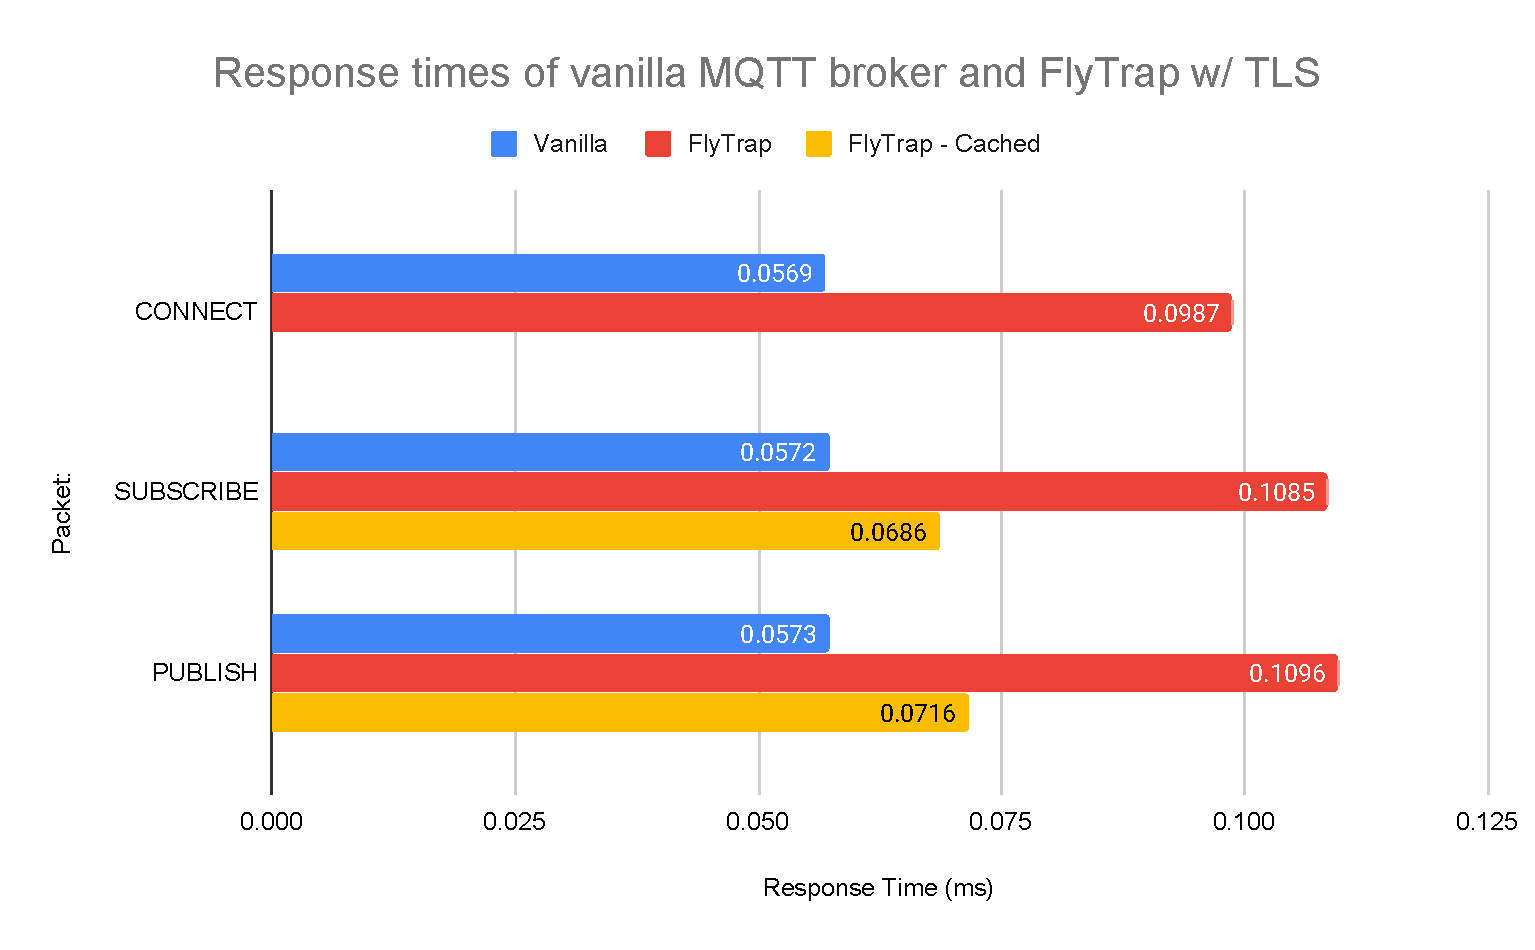
\includegraphics[width=\textwidth]{latency_tls}
    \caption{Response times of most common MQTT requests connection with SSL/TLS encryption}
    \label{fig:latency_tls}
\end{figure}

Statistical tests have been performed on all three datasets. Each of the 100 results for every packet has been compared with the counterpart, for example 100 CONNECT reponse times via Vanilla Broker vs 100 CONNECT reponse times via FlyTrap. This allows us to reject the null hypothesis, as for first test the \textit{p-value} is $<0.05$. Tests number 2.\ and 3.\ resulted with \textit{p-value} $=0$, which can be interpreted as significantly lower than 0.001.

\begin{table}[h]
\centering
\begin{tabular}{|l|l|l|l|}
\hline
\textbf{\#} & \textbf{Test Data}                       & \textbf{Performed Test} & \textbf{p-value}                      \\ \hline
1           & CONNECT: Vanilla vs FlyTrap              & Two Tailed T-Test       & $2.16*10^{-69}$                    \\ \hline
2           & SUBSCRIBE: Vanilla vs FlyTrap vs Cached & Kruskal-Wallis          & $<<< 0.001$ \\ \hline
3           & PUBLISH: Vanilla vs FlyTrap vs Cached & Kruskal-Wallis          & $<<< 0.001$ \\ \hline
\end{tabular}
\caption{Outcome of statistical tests on each the MQTT packets considered for TLS-encrypted connection}
\label{tab:ttest-tls}
\end{table}
\subsection{Plain TCP}

Test above has been repeated, this time disabling TLS encryption for both ends of the connection. First thing that we can notice is the overall decrease of response times, when compared with TLS connection. This is a clear indicator that TLS indeed adds an overhead to standard TCP connections. Experiment results were placed on a barchart in a similar manner as before. Again, standard error bars were omitted, as they were found to be less than $0.01\%$.

Figure \ref{fig:latency_notls} shows the average response time for each of the packets. When sending the request through FlyTrap, we notice an increase in response time of $18.13\%/43.30\%/31.58\%$ respectively for CONNECT/SUBSCRIBE/PUBLISH packets. For FlyTrap - Cached, when compared with Vanilla, this increase less prominent, showing an increase of $23.41\%/15.55\%$ respectively for SUBSCRIBE/PUBLISH packets. 
\begin{figure}[h]
    \centering
    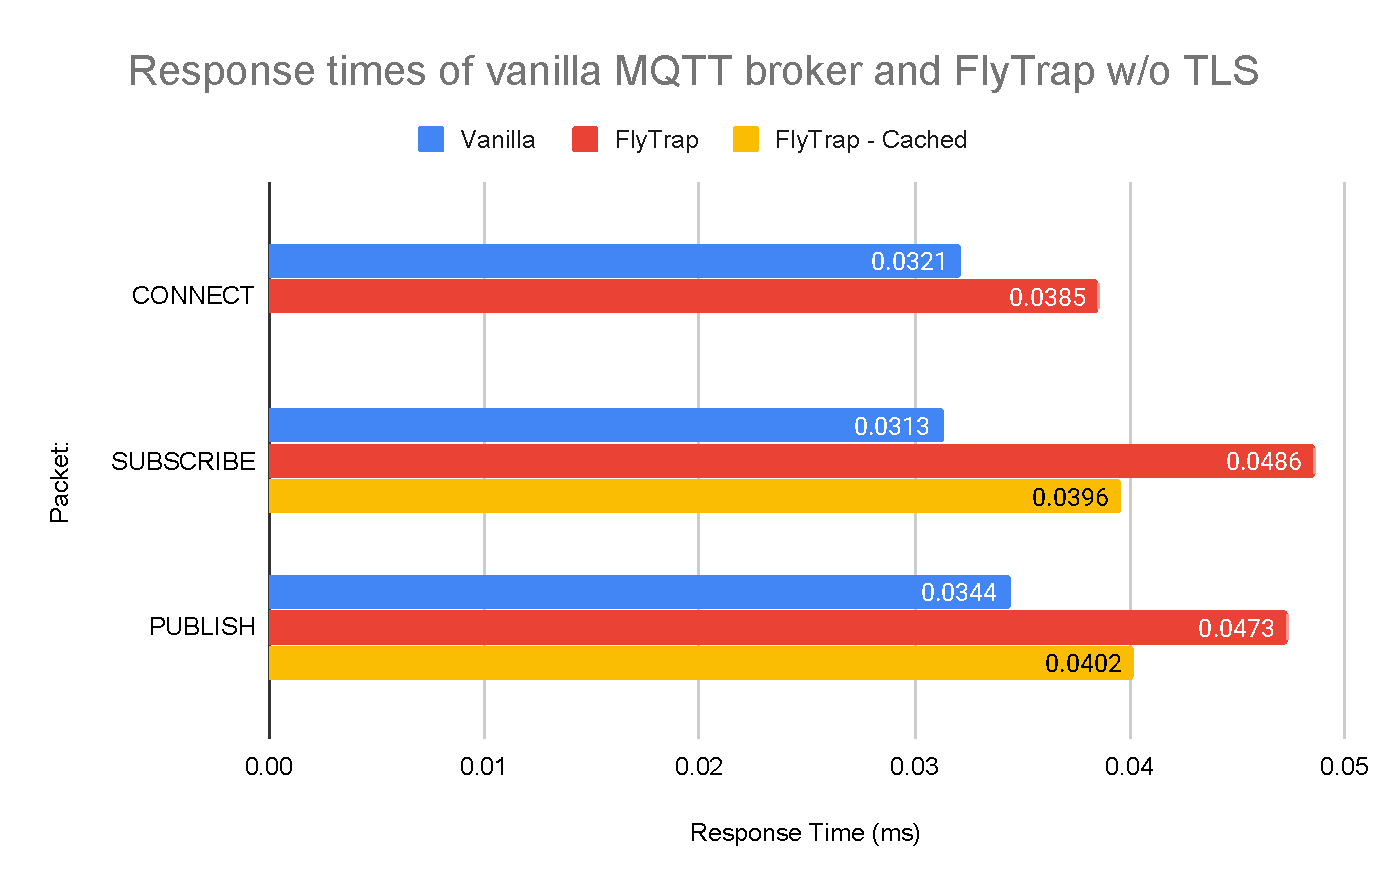
\includegraphics[width=\textwidth]{latency_notls}
    \caption{Response times of most common MQTT requests on plain TCP connection}
    \label{fig:latency_notls}
\end{figure}

In order to deem the results statistically significant, I performed identical tests as in TLS-focused experiment. For each of the tests, the \textit{p-value} was found to be $<0.05$ thus allowing me reject the null hypotheses. Table\ \ref{tab:ttest-notls} shows the specific values of performed statistical tests.

\begin{table}[h]
\centering
\begin{tabular}{|l|l|l|l|}
\hline
\textbf{\#} & \textbf{Test Data}                       & \textbf{Performed Test} & \textbf{p-value}                      \\ \hline
1           & CONNECT: Vanilla vs FlyTrap              & Two Tailed T-Test       & $8.60*10^{-20}$                    \\ \hline
2           & SUBSCRIBE: Vanilla vs FlyTrap vs Cached & Kruskal-Wallis          & $<<< 0.001$ \\ \hline
3           & PUBLISH: Vanilla vs FlyTrap vs Cached & Kruskal-Wallis          & $<<< 0.001$ \\ \hline
\end{tabular}
\caption{Outcome of statistical tests on each the MQTT packets considered on plain TCP connection}
\label{tab:ttest-notls}
\end{table}


\section{Scalability Evaluation}
To perform this test, 100/1000/10000 concurrent clients will be dispatched to PUBLISH a single message, with identical size across all tests, through FlyTrap with TLS enabled. Every client will be dispatched at the same time, as a separate process, thus ensuring that they do not interfere with each other. Each will be identifying with a different Public Key, forcing FlyTrap to perform authentication flow. Then, time when PUBACK has been received will be captured and saved.

\begin{figure}[h]
    \centering
    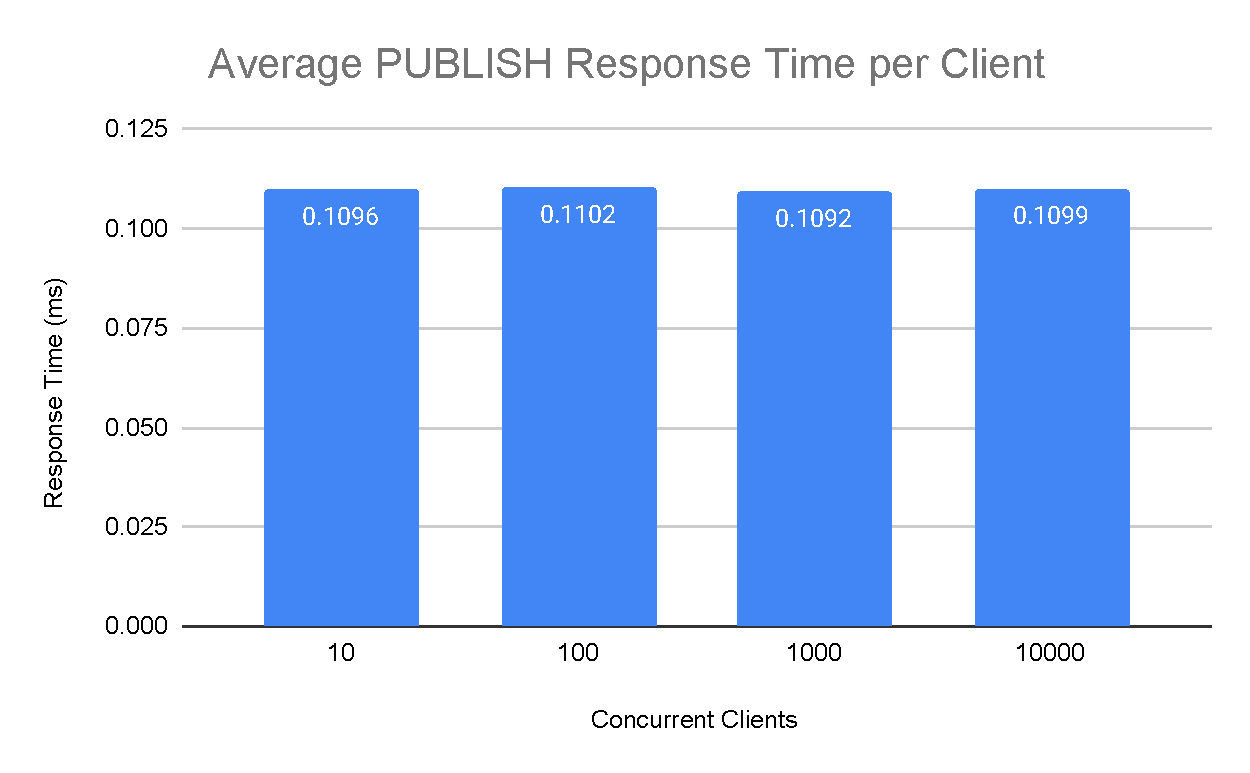
\includegraphics[width=0.8\textwidth]{scale}
    \caption{Average response times with regards to number of concurrent clients}
    \label{fig:scale}
\end{figure}
See figure \ref{fig:scale} with the outcome. We can see that the response time remains constant across a different number of concurrent clients, with less than $1\%$ change between tests.

\section{Cost Evaluation}
As mentioned, Proof-of-Authority networks do not have any currency involved and thus there is no reward for mining. But this removes the benefits of transparency and publicity of the data. On the other hand, running it on a public network (a.k.a. Proof-of-Stake), where miners compete to add new blocks to the network, involves fees and payments and it's important to keep this cost to the minimum.

\begin{figure}[h]
    \centering
    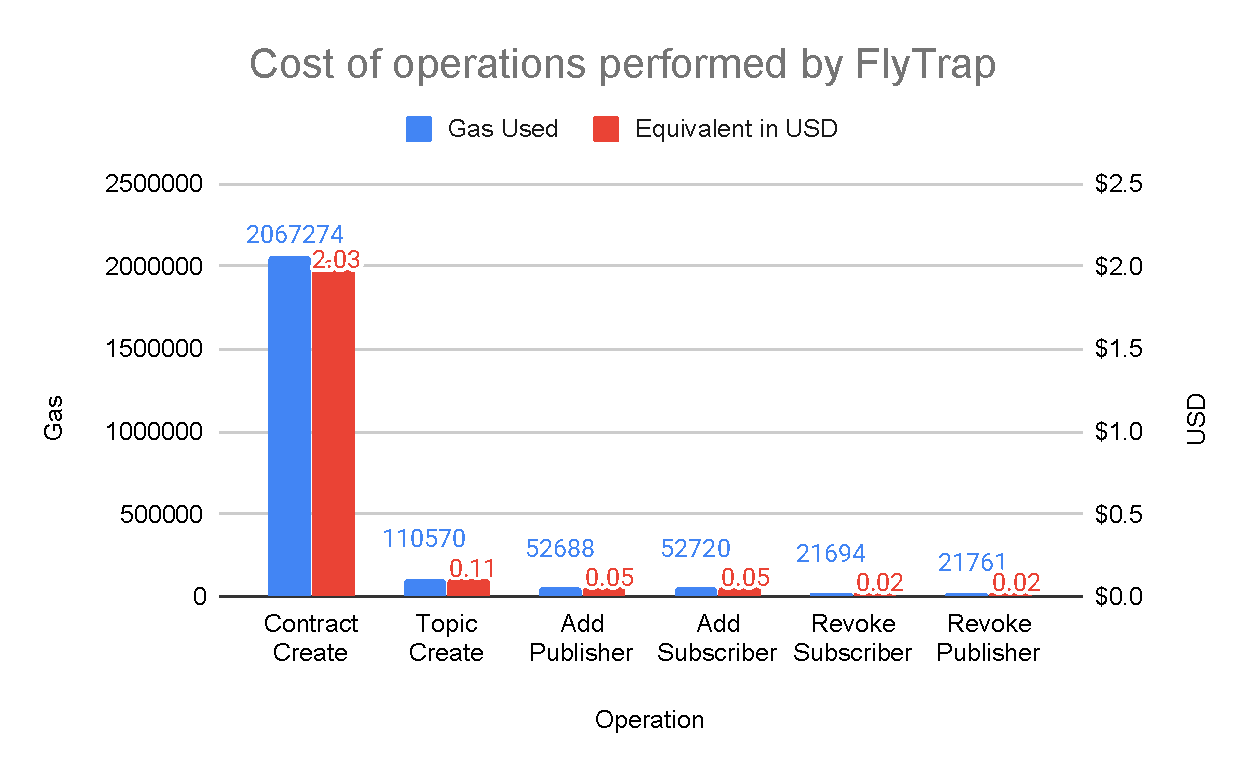
\includegraphics[width=\textwidth]{cost}
    \caption{Cost comparison of various operations on blockchain}
    \label{fig:cost}
\end{figure}

Six operations performed by FlyTrap were executed a hundred times to extract the average costs in gas. To put those numbers into a perspective, I have also included the equivalent value in USD - assuming relations of 1 ETH = \$182.29 and 1 Gas = 0.0000000054 ETH\footnote{Data from https://ethgasstation.info/ and https://cex.io/eth-usd as of 2020-04-18}


\section{Scenarios Evaluation}
In the last test for the evaluation we will be looking at verifying whether the produced software meets the defined requirements in chapter 3. This will focus mostly on a walk-through each of the scenarios, demonstrating how the implemented features satisfy the business need defined in the user story.

Scenario \#5 has been omitted, as the security aspect will be apparent through the remaining tests.
\subsection{Setup}
Each of those scenarios will share common setup steps, which will setup the initial network and proxy. I am going to walk through those steps here - which then can be assumed to be executed prior to any of the subsequent scenarios.
\paragraph{Step 1} - configure your blockchain. For the sake of this experiment, I'm going to use Ganache, which will start a test network, with accounts that have 100 ETH pre-filled currency. Once started, you should obtain a window similar to figure \ref{fig:ganache}.
\paragraph{Step 2} - set endpoint for your blockchain node (Ganache default) and create a new contract for FlyTrap.
\begin{lstlisting}[language=bash]
$ export BLOCKCHAIN_ADDRESS="http://localhost:7545"
$ go run cmd/blockchain/main.go -new -contract=""
2020/04/18 20:28:44 Generated new contract, address is:
0xD0BaD0f1fC6D627E1e6fcE6020De9BbA2507498f
\end{lstlisting}
\paragraph{Step 3} - set contract as environmental variable, add new topic and add publishers/subscribers.
\begin{lstlisting}[language=bash,breaklines=true]
$ export BLOCKCHAIN_CLIENT="0xD0BaD0f1fC6D627E1e6fcE6020De9BbA2507498f"
$ go run cmd/blockchain/main.go -new_topic "creating test topic" -topic "TopicName"
$ go run cmd/blockchain/main.go -topic "TopicName" -client "<client_pubkey>" -pub "adding test publisher"
$ go run cmd/blockchain/main.go -topic "TopicName" -client "<client_pubkey>" -sub "adding test subscriber"
\end{lstlisting}
\paragraph{Step 4} - start web server. Now you should be able to access the website under localhost:8081.
\begin{lstlisting}[language=bash,breaklines=true]
$ go run webapp/main.go
\end{lstlisting}
\paragraph{Step 5} - finally, we are ready to start our FlyTrap proxy. The command will assume TLS as default, with summary reports generated every hour, connection to test mosquitto broker and starts accepting connections under port 8888.
\begin{lstlisting}[language=bash,breaklines=true]
$ go run cmd/flytrap/main.go -b-freq=1h
2020/04/18 21:04:15 Now accepting connections under :8888
\end{lstlisting}
\subsection{Scenario \#1}
For this scenario, we are looking to restrict access to a specific topic, only to people connecting from country which has been permitted. To do so, we will need to slightly modify step 2 from the setup process adding an extra `country' flag to the command, as follows:
\begin{lstlisting}[language=bash,breaklines=true]
$ export BLOCKCHAIN_CLIENT="0xD0BaD0f1fC6D627E1e6fcE6020De9BbA2507498f"
$ go run cmd/blockchain/main.go -new_topic "creating test topic" -topic "RestrictedTopic" -country="GB"
\end{lstlisting}
From now on, only people connecting from British IPs will be allowed, everyone else will be presented with the following message:
\begin{lstlisting}[language=bash,breaklines=true]
$ go run client.go -pub=20 -tls=false -priv="privkey1.asc"
2020/04/18 21:04:17 Using cached signature & public key
2020/04/18 21:04:17 Publishing message: Here Be Dragons #0
panic: error publishing: The PUBLISH is not authorized.
\end{lstlisting}
\subsection{Scenario \#2}
This scenario requires us to determine who access the requested resource on the specific day, so we can determine the scope of the leak. Once the steps in the setup have been completed (in particular, we are about `freq' option) and the leak happens, we are ready to inspect the website.

\begin{figure}[h]
    \centering
    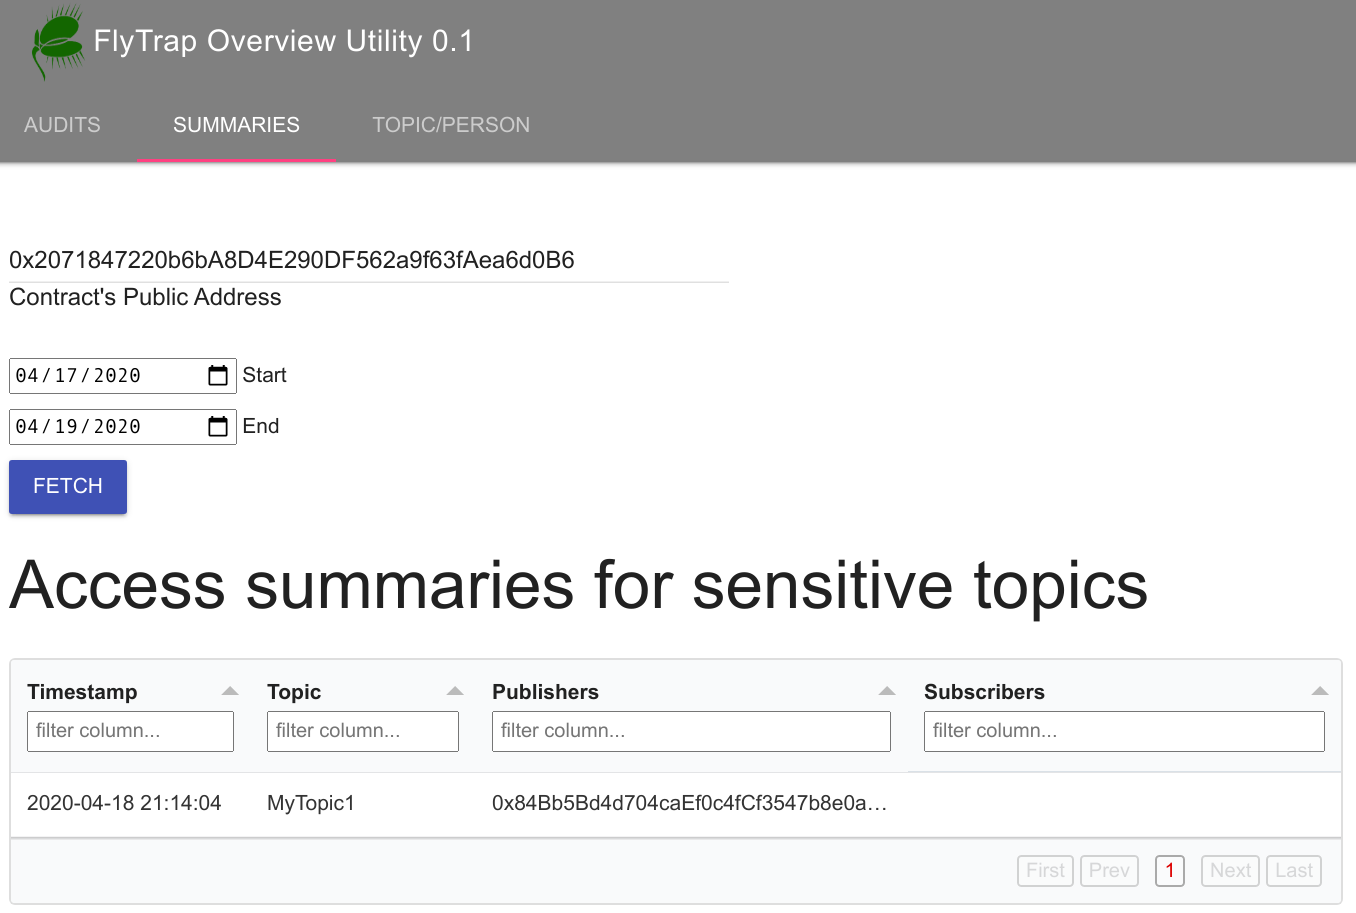
\includegraphics[width=0.9\textwidth]{scenario2}
    \caption{Sensitive topics report}
    \label{fig:scenario2}
\end{figure}
Figure \ref{fig:scenario2} shows how the website would look like upon inspecting the access summaries. We can see that on April 18th in the evening, topic `MyTopic1' was accessed by a single person with the shown public key. Now, we are able to trace the leakage down to a single person and verify whether their credentials were compromised to further assess the damages.
\subsection{Scenario \#3}
Here we are just looking at verifying who can access particular resource, as we want to ensure that all systems that could have read relevant data have been wiped. Again, after following setup steps, we can go ahead and inspect "Topic/Person" part of the webapp, which would allow us to see a list of public keys that can access given topic, as per figure \ref{fig:scenario3}. Then, the system administrator would be able to correlate public key with the piece of infrastructure accessing the information and ensure that the access is revoked along with 
\begin{figure}[h]
    \centering
    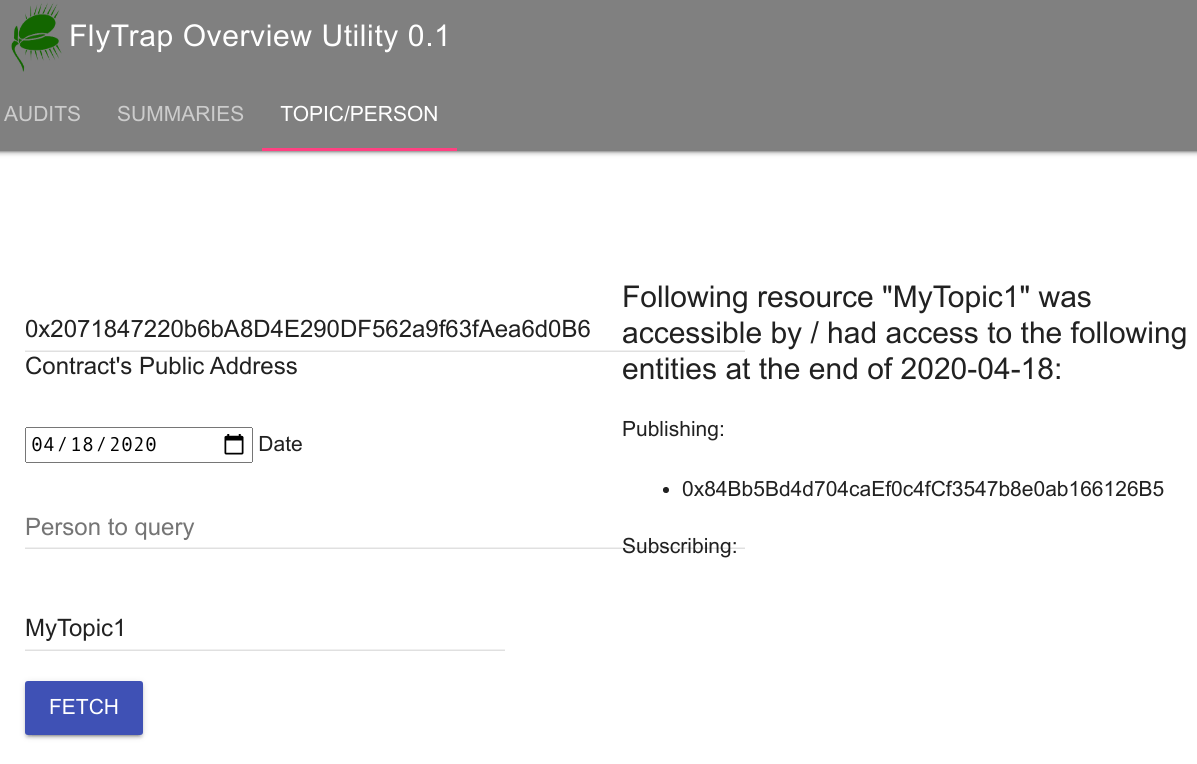
\includegraphics[width=0.9\textwidth]{scenario3}
    \caption{Current Access Control List summary}
    \label{fig:scenario3}
\end{figure}
\section{Results}
\subsection{Latency Evaluation}
The added overhead added by FlyTrap is apparent, reaching even an extra 0.05ms per request. Though, it is interesting to see - looking at ``FlyTrap - Cached'' bar - that caching remediates this problem almost completely, reducing the average response time by up to 37\%, negating the overhead introduced by the first request. We can conclude that FlyTrap would be the most efficient for situations where it is not restarted very often, allowing the cache to grow and in order minimising the impact for clients often connecting to the broker. As expected - we also note longer response time for FlyTrap with TLS enabled. This is most probably caused by the fact that now there need to be two separate TLS sessions established, encrypting/decrypting the data twice.

For FlyTrap with enabled caching functionality, we can notice an average increase of 0.009ms across both plain TCP and TLS when compared with vanilla broker. This is significantly less than specified 500ms in \textbf{NFR1} and thus meets this non-functional requirement and concludes the first research question.

It is also interesting to see that the increased latency is much bigger in TLS connections, when compared to TCP. With TLS, not only we have to deal with an extra overhead of having to contact blockchain to read authentication data, but also perform TLS encryption/decryption twice - first time when communicating with the client and the second time when communicating with the broker.
\subsection{Scalability Evaluation}
On the tested machine, the response times remained constant, indicating that the proxy is capable of handling many concurrent clients without significant impact on performance. If desired, multiple FlyTrap instances can also be deployed across many machines - each pointing to the same broker, further enhacing the response times. This concludes the second research question.

It is important to note that FlyTrap will have an overall limit of maximum allowed concurrent connections of 65535 (equal to $2^{16}$) This is enforced by two limitations. First, MQTT Protocol can only accept Client IDs of at most $2^{16}$ characters long, so naturally it won't be able to proxy more connections than that, since Broker would staright up refuse them. Secondly, FlyTrap operates on linux TCP ports. And again, allowed port range only goes up to 65535. Where the latter problem could be fixed with WebSockets (discussed in the next chapter), the former would still remain a limitation.
\subsection{Cost Evaluation}
For the cost evaluation, the most expensive operation would be creation of the new contract, coming down to \$2.03. Contract contains the bare-bone definition of structures used by FlyTrap, so high price was expected. Though, this only needs to be performed once - the contract can be reused for as many topics as it is necessary. The remaining operations (which would be also performed more often), have their prices much lower. A company looking to create 10 topics with 100 publishers would be looking at an investment of $10 * \$0.11 + 100 * \$0.05 = \$6.1$. This scales linearly and cost remains the same, regardless the current size of the contract and amount of pre-existing topics/publishers/subscribers.

Blockchain offers a solution with 100\% uptime - and at the same time allowing for potential monetisation of accessing the data. The average cost is significantly higher, when compared to centralised solutions, such as SQL server hosted in cloud - but it lacks the benefits of a distributed ledger. Ultimately, all pros and cons would need to be considered before making a decision to utilise Ethereum as a data layer.
\subsection{Scenario Evaluation}
By walking through each of the scenarios, I was able to prove that the software fulfills the business need specified at the beginning of this paper. Scenario's \#4 use-case has been shown to be satisfied through the previous examples, as bare security benefit is considered. For the Scenario \#5, please refer to the User Manual for an explanation on how to set a cost on addining new publishers or subscribers.
